This chapter provides a high-level overview of requirements engineering, requirements tooling, ReqIF and the terminology.

% ===================================================================================
\section{Requirements Engineering \& Management}
\label{sec:requirements_engineering}
\index{requirements engineering}
% ===================================================================================

This book is concerned with \pror{} a tool for requirements engineering.

\begin{definition}{Requirements Engineering}
\index{requirements engineering}
``Requirements engineering (RE) refers to the process of formulating, documenting and maintaining software requirements.'' (\href{http://en.wikipedia.org/wiki/Requirements_engineering}{Wikipedia}).

Requirements are typically recorded in unstructured natural language. However, it is possible to use a formal language as well. Of high interest these days is model-driven requirements engineering.
\end{definition}

But engineering the requirements is not enough: they need to be \textit{managed}.

\begin{definition}{Requirements Management}
\index{requirements management}
``Requirements management is the process of documenting, analyzing, tracing, prioritizing and agreeing on requirements and then controlling change and communicating to relevant stakeholders. It is a continuous process throughout a project.'' (\href{http://en.wikipedia.org/wiki/Requirements_management}{Wikipedia}).
\end{definition}

% ===================================================================================
\section{Tools}
\label{sec:re-tools}
\index{tools}
% ===================================================================================

There are many tools available for requirements engineering.  These include free or cheap ones, like Microsoft Word and Excel, Wikis and issue trackers.  There are expensive, professional ones available, like IBM\textregistered{} Rational\textregistered{} DOORS\textregistered{}, PTC Integrity or Visure IRQA.  Lately, there are also web-based tools, like Siemens Polarion.

\pror{} falls into the category of free tools.  But compared to the ones mentioned, it contains important features from professional tools, including traceability and typed attributes.  Further, by taking advantage of the Eclipse ecosystem, the tool can be augmented by plug-ins for version support, model integration and much more.

\begin{info}
  Professional support, commercial components and integration services are available from \href{http://formalmind.com}{Formal Mind}, via a \href{https://reqif.academy}{ReqIF Academy premium membership}.
\end{info}

% ===================================================================================
\section{Requirements Interchange Format (ReqIF)}
\label{sec:reqif}
\index{ReqIF}
\index{Requirements Interchange Format}
% ===================================================================================

\term{ReqIF} stands for Requirements Interchange Format.  It is an exchange format for requirements and a data model.  \pror{} is an editor that can directly view and modify ReqIF data.

ReqIF was created to support the exchange of requirements across organizations.  For instance, it allows a manufacturer to send requirements to suppliers.  The suppliers can then comment and review the requirements, or they can create a system specification that is linked to the requirements.

ReqIF is an \href{http://www.omg.org/spec/ReqIF/}{official OMG standard}.

\begin{warning}
ReqIF uses its own terminology.  Section~\ref{sec:terminology} defines the ReqIF vocabulary and how it relates to the terms used in classical requirements engineering.
\end{warning}

% -----------------------------------------------------------------------------------
\subsection{ReqIF History}
\label{sec:history}
\index{history}
% -----------------------------------------------------------------------------------

For technical and organizational reasons, two companies in the manufacturing industry are rarely able to work on the same requirements repository and sometimes do not work with the same requirements authoring tools.  A generic, non-proprietary format for requirements information is required to cross the chasm and to satisfy the urgent industry need for exchanging requirement information between different companies without losing the advantage of requirements management at the organizations' borders.

The Requirements Interchange Format (ReqIF) described in this RFC defines such a tool-independent exchange format.  Requirement information is exchanged by transferring XML documents that comply to the ReqIF format.

In 2004, the HIS (Hersteller Initiative Software), a panel of Germany's automotive manufacturers (Daimler, VW, Porsche, Audi and BMW Group) developed the idea of creating the ``Requirements Interchange Format''.  In 2005, the first version of that format was presented at the REConf, a conference about requirements engineering and management, in Munich.  In 2008, the HIS Steering Committee decided that the internationalization and maintenance of the Requirements Interchange Format should be proceeded with the ProSTEP iViP Association.  A project was set up and a team was built that includes members of the ProSTEP iViP Association, representatives of manufacturing companies (Audi, BMW  Group, Daimler, VW, Bosch and Continental), tool vendors (Atego, IBM, MKS) and development partners (HOOD GmbH, PROSTEP AG).

\begin{info}
Further reading: \href{https://reqif.academy/faq/his-process/}{The HIS Exchange Process for Requirements–all you ever wanted to know} at ReqIF.academy.
\end{info}

The ReqIF team expects that making the Requirements Interchange Format an OMG standard increases the number of interoperable exchange tool implementations on the market, fosters the trust of companies exchanging requirement information in the exchange format and provides safety of investments to tool vendors.

% -----------------------------------------------------------------------------------
\subsection{Previous Versions of ReqIF}
\index{RIF}
\label{sec:RIF}
% -----------------------------------------------------------------------------------

This document is submitted as RFC of the Requirements Interchange Format (ReqIF) to the OMG.  Before the submission, the Requirements Interchange Format has been a specification proposed by the HIS and in its latest version, a recommendation of ProSTEP iViP.  For these versions, the abbreviation ``RIF'' has been applied.  The HIS released the Requirements Interchange Format as RIF 1.0, RIF 1.0a, RIF 1.1; RIF 1.1a and the ProSTEP iViP released the recommendation RIF 1.2.

As the acronym RIF has an ambiguous meaning within the OMG, the acronym ReqIF has been introduced to separate it from the W3C`s Rule Interchange Format.  ReqIF 1.0 is the direct successor of the ProSTEP iViP recommendation RIF 1.2.

\begin{warning}
The \pror{} user interface does not currently support RIF.
\end{warning}

% -----------------------------------------------------------------------------------
\subsection{Internal Attributes}
\label{sec:reqif_internal_attributes}
\index{internal attributes}
\index{attributes!internal}
% -----------------------------------------------------------------------------------

ReqIF allows users to define the attributes that SpecObjects may carry.  In addition to these, there are a number of internal attributes that are defined by the ReqIF standard.  Examples include an internal ID or the last change timestamp.

These internal attributes are rarely of interest to users who just want to work with requirements.  However, they may be of interest to tool experts, or may be inspected for troubleshooting.

Internal attributes can be accessed from the Properties View, using the \menu{All Attributes} tab.

% ===================================================================================
\section{Terminology}
\label{sec:terminology}
\index{terminology}
% ===================================================================================

Working with \pror{} can be confusing as it uses the terminology from ReqIF.  For instance, ReqIF uses \textit{SpecObject}s, rather than \term{requirements}.  In the following, we define the more important terms.  More are defined throughout the document.  You can use the index to find the definition of terms.

\begin{info}
This book uses ReqIF terminology throughout.  Please refer to this chapter to understand the meaning of these terms.
\end{info}

A \term{ReqIF model} is the data structure that holds all the information together.  In practical terms, it's just a file, that usually ends in \menu{.reqif} or \menu{.reqifz}.  It contains not just the requirements, but also the data types of those requirements and a lot of other stuff.  It has been described in detail in Section~\ref{sec:reqif}.

\begin{definition}{ReqIF}
\index{ReqIF}
\index{ReqIF Archive}
\index{.reqif}
\index{.reqifz}
\index{Requirements Interchange Format}
ReqIF is an XML-based format for requirements, intended to be used as an exchange format.  It is an open OMG standard and described in detail in Section~\ref{sec:reqif}. The XML data is typically stored in a with with the extension \menu{.reqif}.  It is also possible to store the ReqIF file together with associated data (embedded objects) or other ReqIF files.  These are then stored in a ZIP archive with the extension \menu{.reqifz}.
\end{definition}

Before defining the most important elements, we will provide a brief overview with a concrete example.

% -----------------------------------------------------------------------------------
\subsection{The Most Important ReqIF Elements}
\label{sec:important_elements}
% -----------------------------------------------------------------------------------

Figure~\ref{fig:spec_example} shows a simple ReqIF model, open in \pror{}.  

\begin{figure}
  \centering
  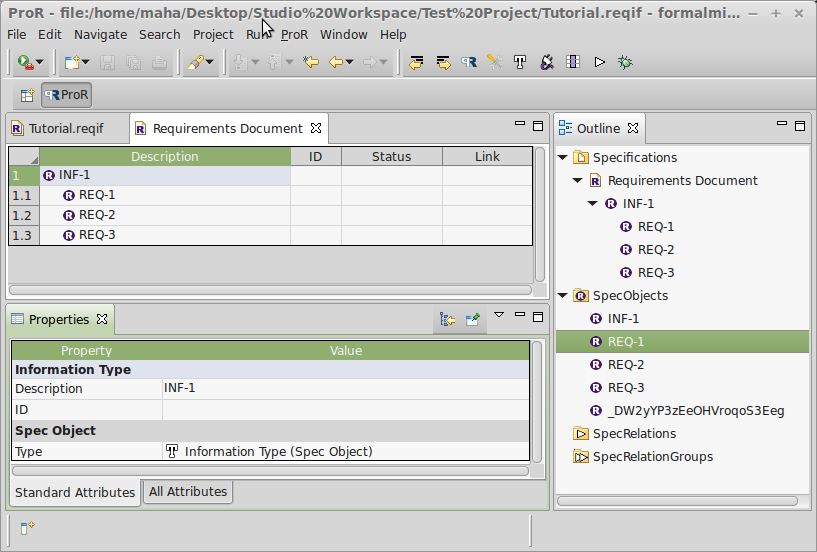
\includegraphics[width=\textwidth]{../rmf-images/screenshot_INF_1.png}
  \caption{Specification example}
  \label{fig:spec_example}
\end{figure}

The \menu{Specification Editor} (the central table) shows the first four \term{SpecObjects}, as visualized in a specification.  The tree-like structure is recognizable: INF-1 is a node
with three children, REQ-1, REQ-2 and REQ-3 (this can be seen by the indentation).  Let's look at INF-1 and REQ-1.  When one is selected in the main pain, it's attributes appear in the \menu{Properties View}, the pane at the bottom.

INF-1 has two \term{Attributes}, ``Description'' and ``ID''.  The \term{SpecType} is ``Information Type'' (shown as the header in the \menu{Properties View}).

REQ-1, REQ-2, and REQ-3 have three Attributes, ``Description'', ``ID'' and ``Status'' (this is not obvious from the figure).  To accommodate this, a column called ``Status'' has been created.  As the ``Information Type'' has no ``Status'' attribute, it is not shown in the \menu{Properties View}.

% -----------------------------------------------------------------------------------
\subsection{SpecElements}
\label{sec:specelements}
\index{SpecElementWithAttributes}
\index{SpecElement}
% -----------------------------------------------------------------------------------

A requirement is called a \term{SpecObject}.  This is arguably the most important element in ReqIF, the actual requirements that you are working with.  The SpecObjects of a ReqIF model can be directly accessed in \pror{} via the outline.  It is more common to access them via a \term{Specification}.  When a SpecObject is selected, its details (attributes and internal information) are shown in the \menu{Properties View}.

\begin{definition}{SpecObject}
\index{SpecObject}
A SpecObject is a data structure for storing requirements information.  It has a number of \term{attributes}.  The most typical attributes include the requirements text and a human-readable ID. A \term{SpecType} determines the attributes of the SpecObject. It is a \term{SpecElement}.
\end{definition}

There are other elements in ReqIF that have a type and attributes.  We call these \term{SpecElements}, although in the official ReqIF specification, they are called \term{SpecElementsWithAttributes}.

\begin{definition}{SpecElement}
\index{SpecElement}
A SpecElement is an abstract ReqIF element that has a \term{SpecType} and \term{Attributes}.  Concrete manifestations include \term{SpecObjects}, \term{Specifications}, \term{SpecRelations} and \term{SpecRelationGroups}.
\end{definition}

Creating links between SpecObjects is a central functionality of requirements tools.  In ReqIF terminology, links are called \term{SpecRelations}.

\begin{definition}{SpecRelation}
\index{SpecRelation}
A SpecRelation is a data structure for connecting two SpecObjects.  It contains a \term{source} and a \term{target} reference to the SpecObjects that are connected.  As a SpecRelation is a SpecElement, it has a type and attributes.
\end{definition}

SpecObjects do not have any particular order.  SpecObjects can be organized into a tree-like structure by using a \term{Specification}.  A Specification is a root element for a tree of SpecObjects.  The SpecObjects are referenced.  This means that the same SpecObject can be referenced multiple times, both within one Specification or in different Specifications.

\begin{definition}{Specification}
\index{Specification}
A Specification is a data structure for organizing SpecObjects into a tree structure.  This tree consists of references.  As a Specification is a SpecElement, it has a type and attributes.
\end{definition}

All SpecElements have a \term{SpecType}.  A SpecType defines \term{AttributeDefinitions}, which defines the attributes for the SpecElement of that type.  

\begin{example}
An AttributeDefinition is just a data type with a label.  Slightly simplified, examples would be:
\begin{itemize}
\item Attribute \term{ID} of type \term{String}
\item Attribute \term{Status} of type \term{Enumeration} with the values \term{accepted} and \term{rejected}
\item Attribute \term{ReqIF.Text} of type \term{XHTML} (rich text).
\end{itemize}
\end{example}

\begin{definition}{SpecType}
\index{SpecType}
The SpecType defines a set of \term{AttributeDefinitions}.  A SpecElement with the given type has the attributes defined by the AttributeDefinitions.
\end{definition}

\begin{definition}{AttributeDefinition}
\index{AttributeDefinition}
An AttributeDefinition belongs to a SpecType. It consists of a label and a DatatypeDefinition, which provides the type.  Some AttributeDefinitions can be configured further.  AttributeDefinitions can also have a \term{default value}.
\end{definition}

Lastly, there are seven \term{DatatypeDefinitions}, some of which can be customized further.

\begin{definition}{DatatypeDefinition}
\index{DatatypeDefinition}
\index{XHTML}
DatatypeDefinitions are the fundamental types in ReqIF and include:

\begin{itemize}
\item
\item Boolean -- true or false
\item Integer -- the range can be customized
\item Real -- range and precision can be customized
\item Date -- also includes the time
\item String -- the maximum length can be customized
\item Enumeration -- both single and multiple choice are supported
\item XHTML -- allow embedding objects of any type
\end{itemize}
\end{definition}

% -----------------------------------------------------------------------------------
\subsection{Comparing Excel and ReqIF}
\label{sec:excel_reqif}
\index{Excel}
% -----------------------------------------------------------------------------------

With the basic terminology in place, we have a quick look at the \pror{} user interface and compare it with Excel.  We do this, as most readers will be familiar with Excel, and it is sometimes used for simple requirements engineering. 

\begin{description}
  \item[Specification.] (Excel-equivalent: Sheet) A ReqIF model can have an arbitrary number of Specifications. In the GUI, it is represented as an Excel-like grid view (see Figure~\ref{fig:spec_example}).

 The \term{Specification} is the ``container'' for the requirements.  Think of an Excel document that allows you to create an arbitrary number of sheets.  Each sheet can be compared to a single Specification.  Most notable differences are: (1) the Specifications are \term{references} rather than independent entities (which means that the same requirement can be referenced and can appear in multiple places); (2) A Specification manages a hierarchy of requirements, while an Excel sheet is a flat list.  This is shown in the Figure, where INF-1 is the parent to three requirements.  The hierarchy is visible both in the main editor, as well as in the outline.

\item[SpecObject.] (Excel-equivalent: Row) A SpecObject represents the actual requirement, and is typically organized in a Specification.

Each row in the Excel spread sheet is the equivalent of a \term{SpecObject}.  A requirement typically has a number of attributes.  Again compared to Excel, each row in a sheet represents a requirement and each cell represents an attribute.  However, in Excel, all rows have the same columns (all requirements have the same attributes), while ReqIF allows mixing SpecObjects of different SpecTypes.  Also, not all attributes need to be shown in a Specification.  

Figure~\ref{fig:spec_example} shows in the \menu{Outline View} a flat list of all SpecObjects.  For instance, the SpecObject \_DW2y... is not referenced in the Specification at all.  Selecting a SpecObject shows its SpecType (in the figure, it is ``Information Type'') and all attributes (in the figure, ``Description'' and ``ID'').

  \item[Attribute.\index{attribute}] (Excel-equivalent: Cell) An attribute holds the actual content of a SpecObject.

In Excel, a new attribute is simply created by putting a column header on a column.  In ReqIF, columns are created via \menu{Studio | Column Configuration}, or by clicking on 
\includegraphics[height=0.8em]{../rmf-images/icons/full/obj16/ProRSpecViewConfiguration.png}.  But content will only be shown if the SpecObject of that row has an attribute of that name.

\index{standard attribute}
\index{attribute!standard}
\index{ProStep Implementor Forum}
Besides the actual text of the requirement, typical attributes include ID, status, etc.  Note that there are no ``standard'' attributes.  However, the ProSTEP Implementor Forum defined a recommendation for a set of standard attributes.

\end{description}


